\documentclass{article}
\usepackage{amsmath}
\usepackage{amssymb}
\newcommand*{\qed}{\hfill\ensuremath{\blacksquare}}
\usepackage{graphicx}
\graphicspath{{.}}
\usepackage{hyperref}
\usepackage{tikz}
\usepackage{pgfplots}
\long\def\/*#1*/{}
\usetikzlibrary{arrows}
\newcommand\tab[1][1cm]{\hspace*{#1}}



\title{Computational Linear Algebra, Module 13}
\author{Maya Shende}
\date{Due: May 2nd, 2018}

\begin{document}
\maketitle

\begin{enumerate}
%exercise 1
\item The dimension of the nullspace is $n-r$. 

%exercise 2
\item Let $A = 
\begin{bmatrix}
a_{11}	&a_{12}	&\dots	&a_{1n}\\
a_{21}	&a_{22}	&\dots	&a_{2n}\\
\vdots	&\vdots	&\ddots	&\vdots\\
a_{m1}	&a_{m2}	&\dots	&a_{mn}
\end{bmatrix}
= 
\begin{bmatrix}
\vdots	&\vdots	&\dots	&\vdots\\
c_1		&c_2		&\dots	&c_n\\
\vdots	&\vdots	&\dots	&\vdots
\end{bmatrix}
$. \\Then, $B = A^TA = \\
\begin{bmatrix}
\dots		&c_1		&\dots\\
\dots		&c_1		&\dots\\
\vdots	&\vdots	&\vdots\\
\dots		&c_n		&\dots
\end{bmatrix}
\begin{bmatrix}
\vdots	&\vdots	&\dots	&\vdots\\
c_1		&c_2		&\dots	&c_n\\
\vdots	&\vdots	&\dots	&\vdots
\end{bmatrix}
= 
\begin{bmatrix}
c_1\cdot c_1	&c_1\cdot c_2	&c_1\cdot c_3	&\dots	&c_1\cdot c_n\\
c_2\cdot c_1	&c_2\cdot c_2	&c_2\cdot c_3	&\dots	&c_2\cdot c_n\\
\vdots		&\vdots		&\vdots		&\ddots	&\vdots\\
c_n\cdot c_1	&c_n\cdot c_2	&c_n\cdot c_3	&\dots	&c_n\cdot c_n
\end{bmatrix}
$ and we know that $c_1\cdot c_2 = c_2\cdot c_1$ (dot product is commutative), therefore we can see that $B$ is symmetric. 

%exercise 3
\item The last step of ${\bf w}_i \cdot {\bf w}_i	= {\bf w}_i^T \cdot {\bf w}_i = \lambda_i {\bf v}_i^T {\bf v}_i = \lambda_i $ is true because we know that the $\textbf{v}_i$ vectors are orthogonal, this $\textbf{v}_i \cdot \textbf{v}_i = 1$ leading to $\lambda_i {\bf v}_i^T {\bf v}_i = \lambda_i$. Therefore, ${\bf w}_i \cdot {\bf w}_i = \lambda_i$.

%exercise 4
\item $V'$ has $n$ rows and $U'$ has $m$ rows

%exercise 5
\item 
\begin{eqnarray*}
AV' \implies (m \times n)(n \times r) = (m \times r)\\
U'\Sigma ' \implies (m \times r)(r \times r) = (m \times r)
\end{eqnarray*}
Therefore the matrix multiplication is size-compatible since the dimensions are the same.


%exercise 6
\item Since $V$ is orthogonal, $V^T = V^{-1}$ and $VV^{-1} = I$. 

%exercise 7
\item Confirmed: \\
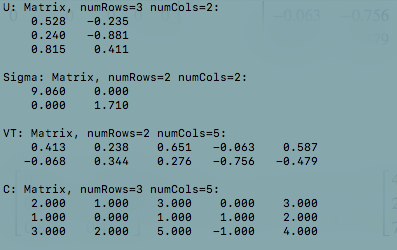
\includegraphics[scale=0.6]{exercise7}

%exercise 8
\item The vector $u_k$ has length $m$ and the vector $v_k$ has length $n$, thus to store the two vectors in memory, it only requires $m+n$ space to store the $m+n$ combined elements of the two vectors. For $p$ such terms, the total storage is $p(m+n)$. Suppose $m = 2$ and $n=3$, then $m \times n = 6$ and $m+n = 5$, so $m+n < m\times n$ when $p =1$, but $m+n>m\times n$ when $p > 1$. Suppose $m = 4$ and $n = 4$, then $m\times n = 16$ and $m+n = 8$, so $m+n \leq m\times n$ when $p \leq 2$ and $m+n > m\times n$ when $p > 2$

%exercise 9
\item There is a very poor approximation with $p=1$\\
$p=1: $\\
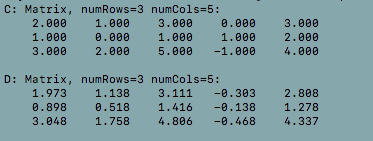
\includegraphics[scale=0.6]{exercise9_p-1}\\
$p=r: $\\
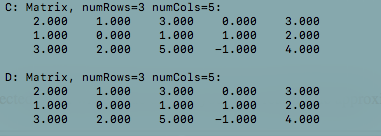
\includegraphics[scale=0.6]{exercise9_p-r}

%exercise 10
\item With $p=10$, we start to see facial features, but with $p=50$, we see a clear image. \\
$p=1: \\$

\includegraphics[scale=0.4]{testimage-1}\\
$p=5: \\$
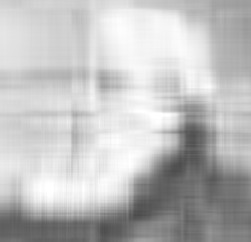
\includegraphics[scale=0.4]{testimage-5}\\
$p=10: \\$
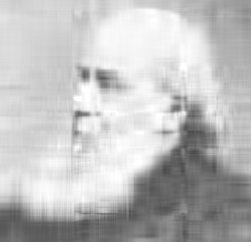
\includegraphics[scale=0.4]{testimage-10}\\
$p=50: \\$
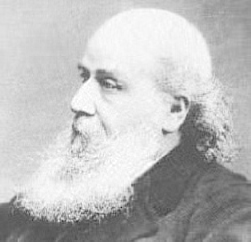
\includegraphics[scale=0.4]{testimage-50}\\
$p=100: \\$
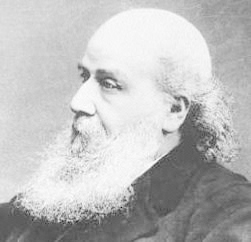
\includegraphics[scale=0.4]{testimage-100}

%exercise 11
\item We are using the $p$ best values, so we are going to get $p$ components instead of all $r$, thus the rank is $p$. Setting the extra $\sigma$ terms to 0 just ensures that those respective terms of $u$ and $v$ are zeroed out as well. 

%exercise 12
\item $U$ is orthogonal, so $U^T = U^{-1}$

%exercise 13
\item Wikinews dataset: \\
$U: (64, 6)$\\
$\Sigma : (6, 6)$\\
$V^T: (6,7)$\\
Covariance computed with changed coordinates shows clustering among the data. \\
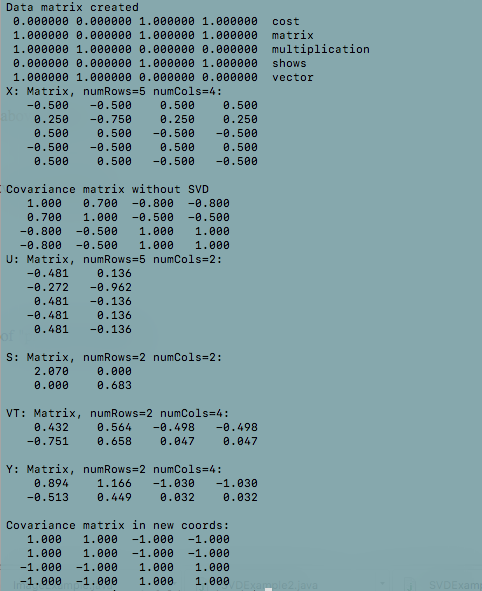
\includegraphics[scale=0.6]{exercise13_1}

%exercise 14
\item The eigen images correspond to the eigen vectors that go into the SVD. They are representative images of the training data. $U: (10000 \times 9)$. \\
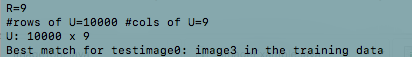
\includegraphics[scale=0.6]{exercise14_1}

%exercise 15
\item $$ {\bf \sum}^{-1} = 
	\begin{bmatrix} 
	\frac{1}{\sigma_1} & 0 & ... & 0 \\
	0 & \frac{1}{\sigma_2} & ... & 0 \\
	\vdots & \vdots & & \vdots \\
	0 & 0 & ... & \frac{1}{\sigma_n}
	\end{bmatrix}$$

%exercise 16
\item Start with $\mathbf{A} = \mathbf{U\Sigma V^T}$. So, 
\begin{eqnarray*}
\mathbf{A} &=& \mathbf{U\Sigma V^T}\\
\mathbf{AV} &=& \mathbf{U\Sigma} \mbox{\tab\tab (since \textbf{V} is orthogonal, $V^T=V^{-1}$)}\\
\mathbf{AV\Sigma^{-1}} &=& \mathbf{U}\\
\mathbf{AV\Sigma^{-1}U^{-1}} &=& \mathbf{I}\\
\mathbf{V\Sigma^{-1}U^{-1}} &=& \mathbf{A^{-1}}
\end{eqnarray*}

%exercise 17
\item This tells us that only the first dimension matters: \\
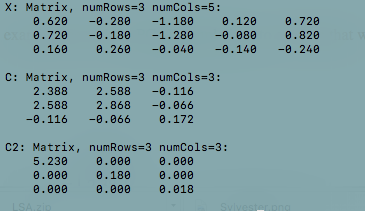
\includegraphics[scale=0.6]{exercise17}

%exercise 18
\item Here we get clusters when running SVD: \\
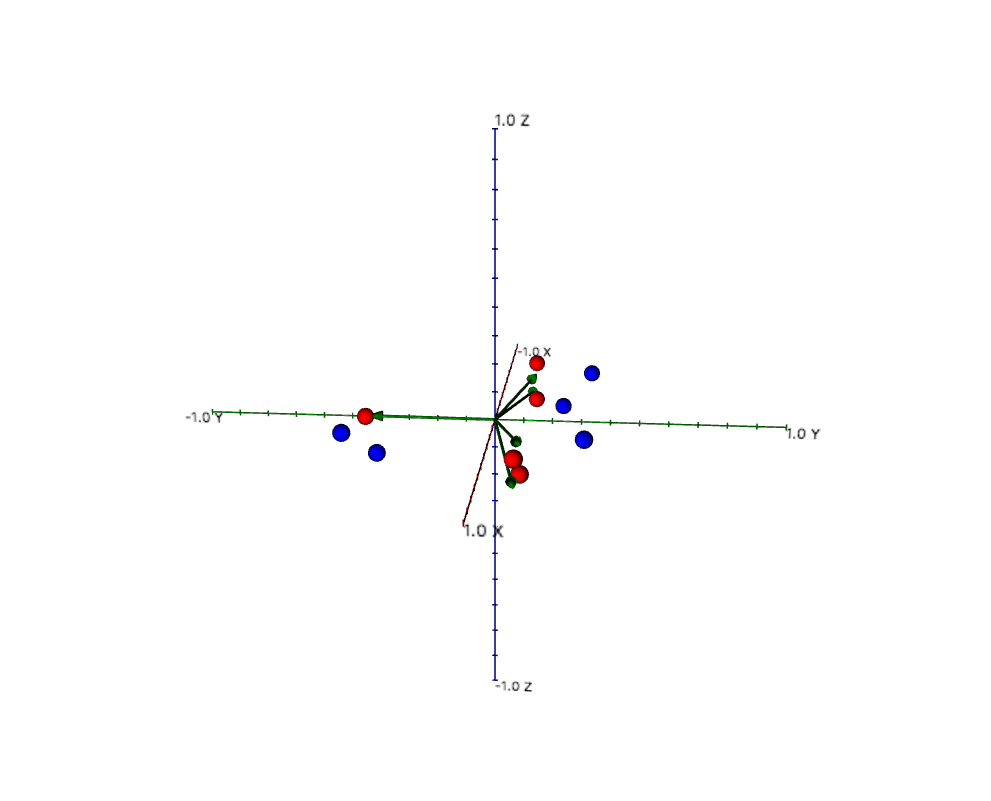
\includegraphics[scale=0.4]{exercise18_plot}\\
Output: \\
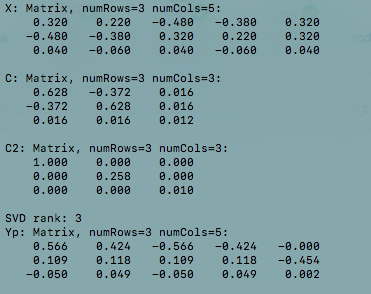
\includegraphics[scale=0.6]{exercise18_output}

\end{enumerate}
\end{document}